% !TEX root = marvin.tex
\begin{figure*}[t]
  \begin{center}
  \iflatexml
  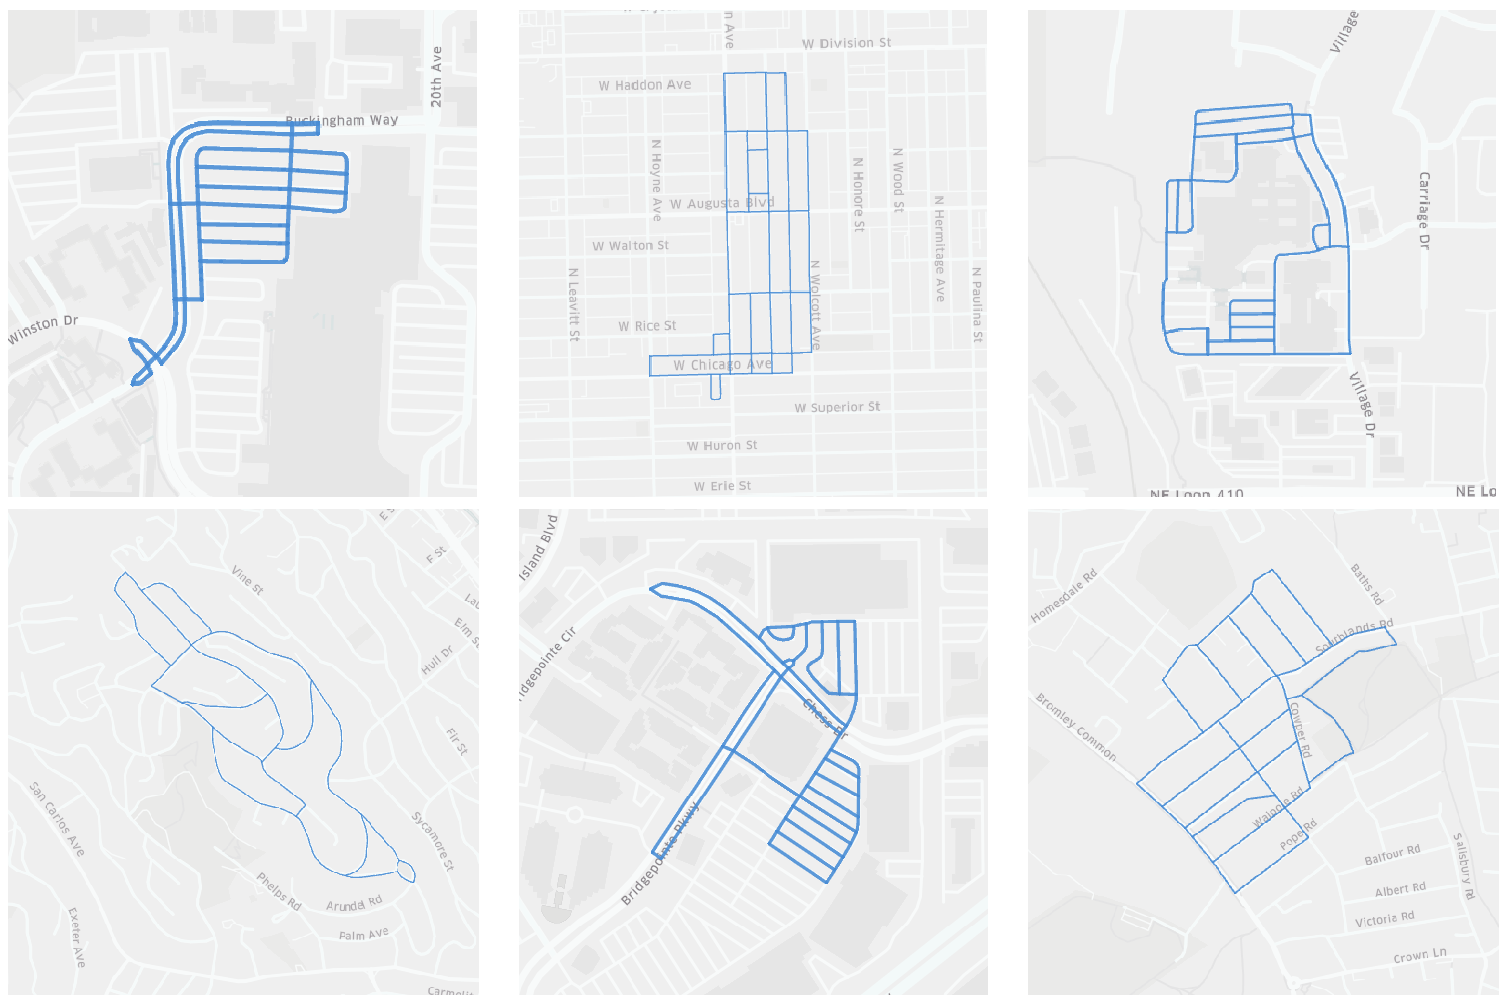
\includegraphics[width=6\textwidth]{figs/example_graphs.png}
  \else
  \begin{tabular}{lll}
    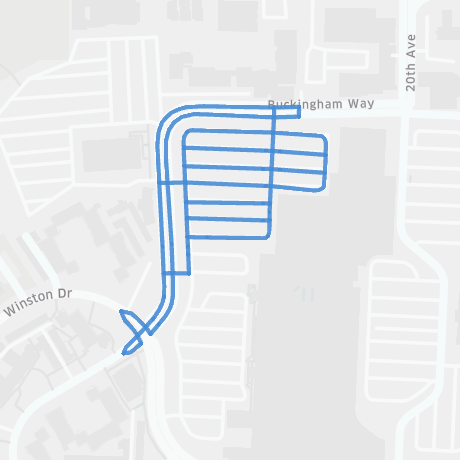
\includegraphics[height=5.1cm,trim={0.2cm 0 0.4cm 0},clip]{figs/graph1.png} &
    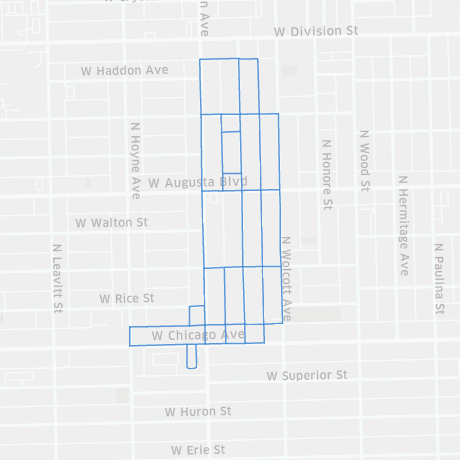
\includegraphics[height=5.1cm,trim={0.2cm 0 0.4cm 0},clip]{figs/graph2.png} &
    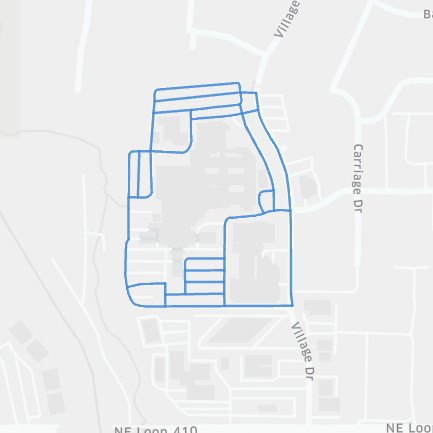
\includegraphics[height=5.1cm,trim={0.2cm 0 0.4cm 0},clip]{figs/graph3.png} \\
    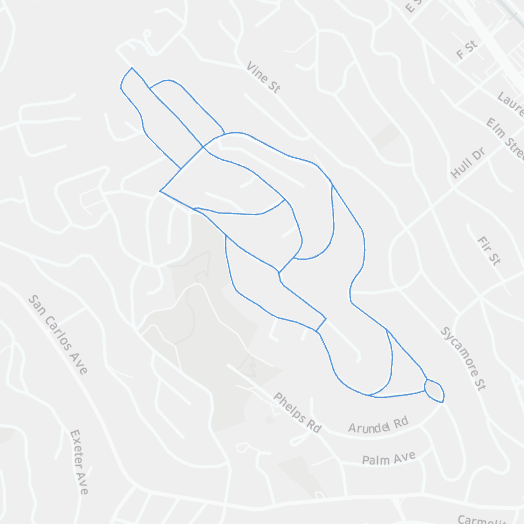
\includegraphics[height=5.1cm,trim={0.2cm 0 0.4cm 0},clip]{figs/graph4.png} &
    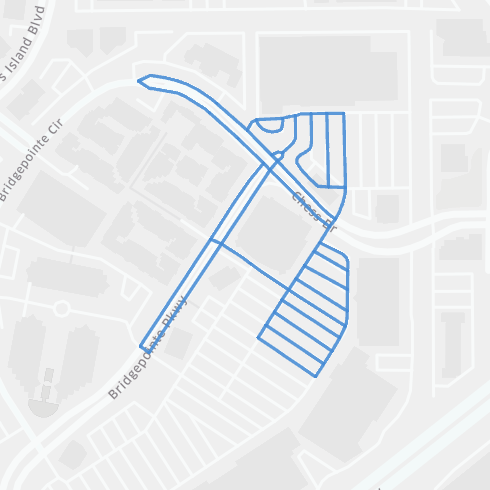
\includegraphics[height=5.1cm,trim={0.2cm 0 0.4cm 0},clip]{figs/graph5.png} &
    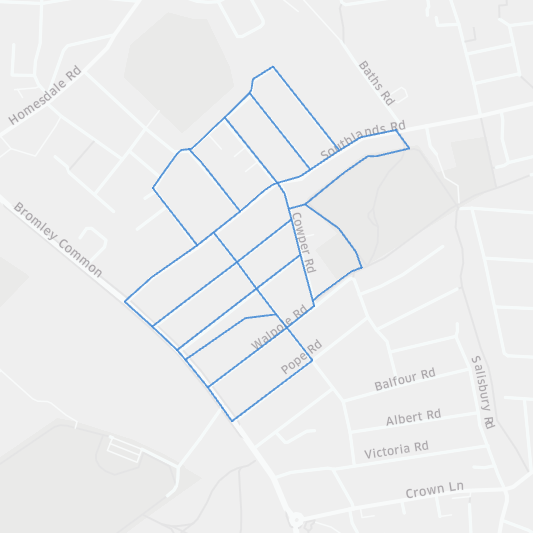
\includegraphics[height=5.1cm,trim={0.2cm 0 0.4cm 0},clip]{figs/graph6.png} \\
  \end{tabular}
  \fi
  % \vspace{-0.15in}
  \caption{Random graphs sampled from the training set. }
  \label{fig:example_graphs}
  \end{center}
  \vspace{-0.25in}
\end{figure*}